\chapter{Implementacija i korisničko sučelje}
		
		
		\section{Korištene tehnologije i alati}
		
 Komunikacija u timu realizirana je korištenjem aplikacije Slack\footnote{\url{https://slack.com/}} koja omogućuje jednostavnu i veoma organiziranu komunikaciju kroz „channel“ i „therad“ mogućnosti komuniciranja. Za izradu UML dijagrama korišten je alat Astah UML\footnote{\url{https://astah.net/products/astah-uml/}}, a kao sustav za upravljanje izvornim kodom Git\footnote{\url{https://git-scm.com/}}. Udaljeni repozitorij projekta dostupan je na web platformi GitLab\footnote{\url{https://about.gitlab.com/}}.

 Kao razvojno okruženje korišten je Visual Studio Code\footnote{\url{https://code.visualstudio.com/}} – integrirano razvojno okruženje (IDE) tvrtke Microsoft\footnote{\url{https://www.microsoft.com/hr-hr/}} koje dolazi sa ugrađenom podrškom za JavaScript\footnote{\url{https://www.javascript.com/}}, TypeScript\footnote{\url{https://www.microsoft.com/hr-hr/}} i Node.js\footnote{\url{https://nodejs.org/en/}} te pruža IntelliSense\footnote{\url{https://code.visualstudio.com/docs/editor/intellisense}} (inteligentno dovršavanje koda obzirom na kontekst), podršku za otklanjanje pogrešaka, refaktoriranje koda, ugrađene naredbe za Git i mnogobrojna proširenja za ostale programske jezike i alate.

 Klijentska strana aplikacije \textit{(frontend)} napisana je koristeći radni okvir Vue.js\footnote{\url{https://vuejs.org/}} zasnovan na JavaScriptu odnosno TypeScriptu (JavaScript s podrškom za tipove) koji pruža učinkoviti razvoj klijentskog sučelja koristeći već dostupne web komponente i predloške.

 Poslužiteljska strana aplikacije \textit{(backend)} napisana je u programskom jeziku TypeScript koristeći radni okvir Express\footnote{\url{https://expressjs.com/}} koji pojednostavljuje proces izgradnje i razvoja web aplikacija koristeći Node.js. Express pruža funkcionalnosti posredničke arhitekture \textit{(middleware)} i usmjeravanja, jedan je od najpopularnijih okvira za Node.js te se široko koristi za izgradnju malih i velikih web aplikacija. Također, korištena je i ORM \textit{(Object-Relational Mapping)} bilblioteka Sequlize\footnote{\url{https://sequelize.org/}} koja omogućuje interakciju s relacijskim bazama podataka koristeći objektno orijentiranu sintaksu, umjesto izravnih SQL upita.

Jednostavno pokretanje, konfiguraciju i puštanje u pogon te neovisnost o računalu na kojem se kod izvršava omogućava korištenje platforme Docker\footnote{\url{https://www.docker.com/}}. Kroz tri Docker kontejnera pokriveni su svi ključni dijelovi/slojevi aplikacije – klijent, poslužitelj i PostgreSQL\footnote{\url{https://www.postgresql.org/}} baza podataka te su osigurane točne verzije svih vanjskih biblioteka i alata.


			\eject 
		
	
		\section{Ispitivanje programskog rješenja}
			
			\textbf{\textit{dio 2. revizije}}\\
			
			 \textit{U ovom poglavlju je potrebno opisati provedbu ispitivanja implementiranih funkcionalnosti na razini komponenti i na razini cijelog sustava s prikazom odabranih ispitnih slučajeva. Studenti trebaju ispitati temeljnu funkcionalnost i rubne uvjete.}
	
			
			\subsection{Ispitivanje komponenti}
Unit testovima provjeravamo ispravnost funkcionalnosti „utils“ funkcija koje su korištene kao pomoćne funkcije na više različitih dijelova koda.
Proveli smo sedam unit testova te u nastavku slijede njihovi kratki opisi i odgovarajući kodovi, na kraju slijedi slika izvođenja rezultata testova.

 \textbf{Ispitni slučaj 1. : Unos e-mail adrese}  

                \textbf{Ulaz:}

                1. Unos ispravne e-mail adrese.

                2. Unos adrese bez domene.

                3. Unos domene bez username-a.

                4. U upisanome e-mailu nedostaje '@'.

                5. Nedostaje točka koja razdvaja domenu i esktenziju.

                6. Nedostaje ekstenzija.

                7. Ekstenzija je predugačka.

                \textbf{Očekivani rezultat:}

                1. Provjera je prošla i e-mail adresa je validna.

                2.-7. Sustav javlja grešku kako je i predviđeno kao cilj ovog testa. 

                \textbf{Rezultat:} 

                Svi testovi su zadovoljeni, aplikacija je prošla test!

	\begin{figure}[H]
			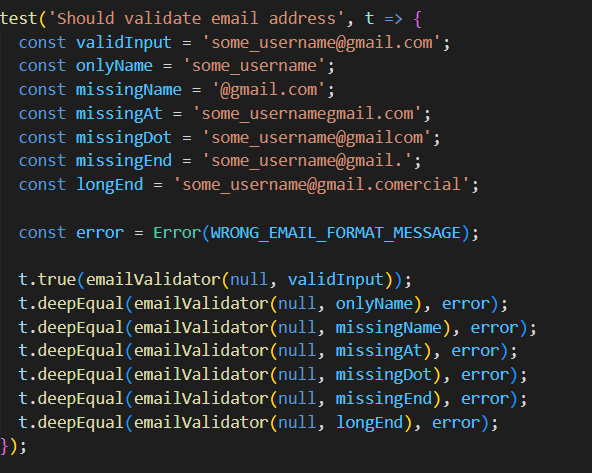
\includegraphics[scale=0.5]{slike/EmailTest.PNG} %veličina slike u odnosu na originalnu datoteku i pozicija slike
			\centering
			\caption{Test unosa e-mail adrese}
			\label{fig:ppp}
			
		\end{figure}

 \textbf{Ispitni slučaj 2. : Funkcija „subtractYears“ – funkcije koja oduzima zadan broj godina od nekog određenog datuma}

U svrhu tog testiranja definiramo novi datum od kojeg ćemo oduzeti zadan broj godina, definiramo očekivani datum te u varijablu spremamo rezultat funkcije. Naredbom „deepEqual“ provjeravamo jesu li rezultat funkcije i očekivana vrijednost jednaki. 

\textbf{Ulaz:}

	1.Slobodno izabran datum, očekivani rezultat funkcije, broj godina koje oduzimamo

 \textbf{Očekivani rezultat:} 

	1. Slobodno izabran datum umanjen za zadani broj godina, provjera je prošla

 \textbf{Rezultat:}  

Svi testovi su zadovoljeni, aplikacija je prošla test!



\textbf{Ispitni slučaj: Funkcija „toDatePicker“ koja zadano vrijeme vraća u milisekundama}

U svrhu tog testiranja definiramo dva datuma čija je vremenska razlika u milisekundama jednaka poznatoj vrijednosti, te provjeravamo rezultat vremenske razlike dvaju datuma pretvorenih funkcijom „toDatePicker“ u milisekunde, ako rezultat funkcije „is“ bude potvrdan, funkcija „toDatePicker“ radi kako je očekivano.

\textbf{Ulaz:}

1.Dva datuma čija je razlika poznat broj milisekundi, poznat broj milisekundi

 \textbf{Očekivani rezultat:}  

1.Rezultat razlike poziva funkcije koja datume pretvara u milisekunde, provjera je prošla

\textbf{Rezultat:} 

 Svi testovi su zadovoljeni, aplikacija je prošla test!

\begin{figure}[H]
			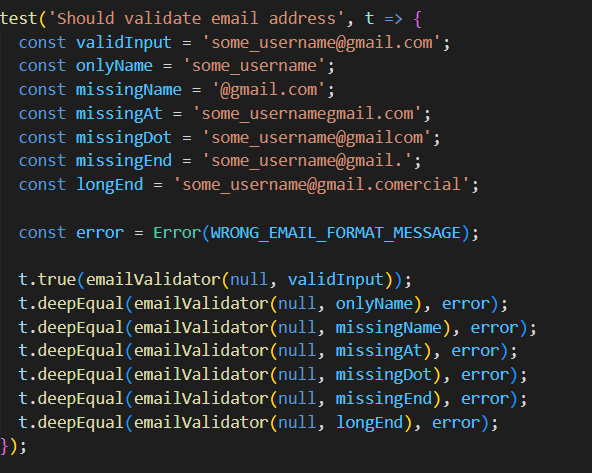
\includegraphics[scale=0.5]{slike/EmailTest.PNG} %veličina slike u odnosu na originalnu datoteku i pozicija slike
			\centering
			\caption{Test unosa e-mail adrese}
			\label{fig:ppp}
			
		\end{figure}


 \textbf{\textit{Ispitni slučaj: provjera zadovoljenosti dobne granice}}\\

            \textbf{\textit{Ulaz:}}\\
            
             1. Korisnik unosi današnji datum u mjesto za unos datuma rođenja

             2. Korisnik unosi datum točno 15 godina stariji od današnjeg

             3. Korisnik unosi datum točno 12 godina stariji od današnjeg

             \textbf{\textit{Očekivani rezultat:}}

             1. Sustav javlja error - uneseni datum rođenja nije dozvoljen!

             2. i 3. Sustav ne javlja error - uneseni datum rođenja je dozvoljen!

             \textbf{\textit{Rezultat:}}

             Svi testovi su zadovoljeni, aplikacija je prošla test!

\begin{figure}[H]
			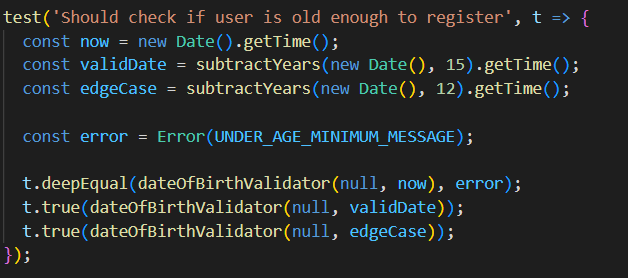
\includegraphics[scale=0.5]{slike/ageTest.PNG} %veličina slike u odnosu na originalnu datoteku i pozicija slike
			\centering
			\caption{Test zadovoljenosti dobne granice}
			\label{fig:aaa}
			
		\end{figure}
	
	 \textbf{\textit{Ispitni slučaj: provjera ispravnosti broja mobitela}}

            \textbf{\textit{Ulaz:}}

             1. Korisnik u odgovarajuće mjesto upisuje broj mobitela sa 9 znamenki

             2. Korisnik u odgovarajuće mjesto upisuje broj mobitela sa 10 znamenki

             3. Korisnik u odgovarajuće mjesto upisuje broj mobitela sa 9 znamenki čije su znamenke odvojene u grupe po 3 koje su razdvojene razmakom

             4. Korisnik u odgovarajuće mjesto upisuje broj mobitela sa 10 znamenki čije su znamenke odvojene u dvije grupe po 3 i jednu grupu po 4 znamenke te su grupe razdvojene znakom 

             5. Korisnik u odgovarajuće mjesto upisuje broj mobitela sa više od 10 znamenki

             6. Korisnik u odgovarajuće mjesto upisuje broj mobitela sa manje od 9 znamenki

             7. Korisnik u odgovarajuće mjesto upisuje broj mobitela koji sadrži slovo

             8. Korisnik u odgovarajuće mjesto upisuje broj mobitela koji sadrži znak 

            \textbf{\textit{Očekivani rezultat:}}

             1. - 4. Sustav ne javlja error - broj mobitela je validan!

             5. - 8. Sustav javlja error - broj mobitela nije validan!

             6. Sustav javlja error - broj mobitela nije validan!

             \textbf{\textit{Rezultat:}}

             Svi testovi su zadovoljeni, aplikacija je prošla test!

\begin{figure}[H]
			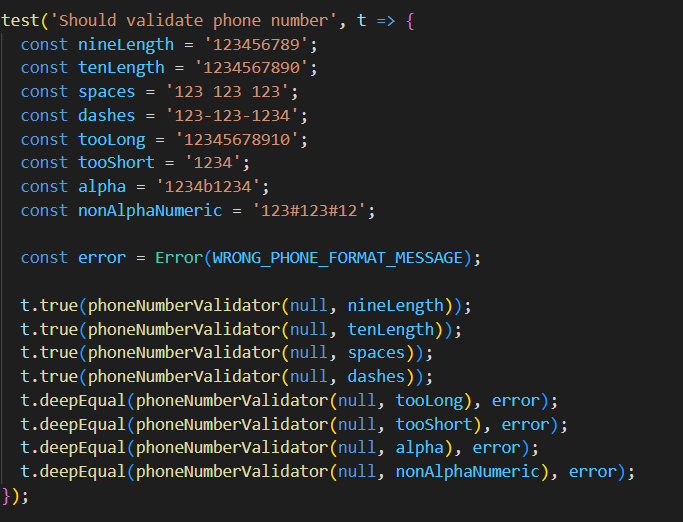
\includegraphics[scale=0.5]{slike/numberTest.PNG} %veličina slike u odnosu na originalnu datoteku i pozicija slike
			\centering
			\caption{Test ispravnosti broja mobitela}
			\label{fig:bbb}
			
		\end{figure}


\textbf{\textit{Ispitni slučaj: provjera valjanosti poslanih url adresa}}

Testiramo kako će aplikacija reagirati kada joj šaljemo raličite url destinacije, odnosno testovima definiramo ispravne destinacije i pogrešne destinacije u kojima je učinjena pogreška ili fali neki logički dio url adrese.
U prva dva slučaja kada je ulaz ispravan test je ispravan, a u ostalim slučajevima testni slučaj ne prolazi.

            \textbf{\textit{Ulaz:}}

             1. i 2. Unos ispravne url adrese     
        
             3. Unos  url adrese bez protokola

	     4. unos url adrese bez dvotočke

	     5. unos url adrese bez /

             6. unos rla adrese bez //

             7. unos url adrese bez .com domene

             \textbf{\textit{Očekivani rezultat:}}

             1. i 2. Sustav ne javlja error - url adresa je ispravna

             3.-7. Sustav  javlja error - url adresa je nesipravna

             \textbf{\textit{Rezultat:}}

             Svi testovi su zadovoljeni, aplikacija je prošla test!

\begin{figure}[H]
			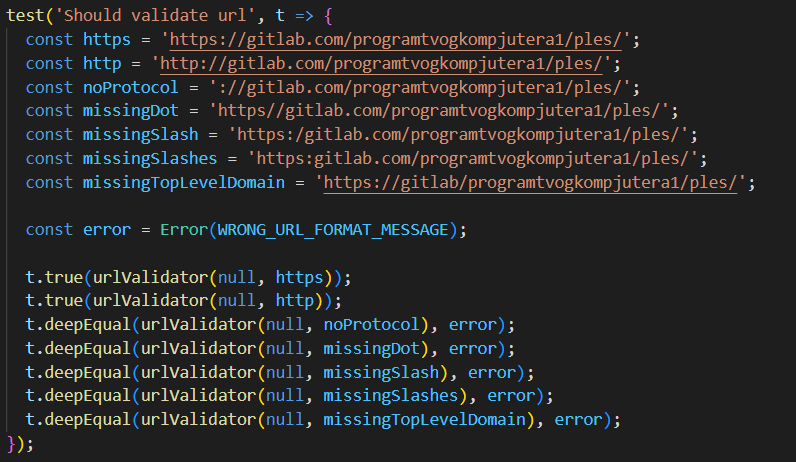
\includegraphics[scale=0.5]{slike/urlTest.PNG} %veličina slike u odnosu na originalnu datoteku i pozicija slike
			\centering
			\caption{Test valjanosti url adresa}
			\label{fig:ajoj}
			
		\end{figure}
			
			
			
			\subsection{Ispitivanje sustava}
			
			\textbf{\textit{Ispitni slučaj 1: provjera ispravnosti logina}}\\
			\textbf{\textit{Ulaz:}}\\
			
			 \textit{1. Korisnik se ulogira u sustav kao user}\\
			 \textit{2. Korisnik se ulogira u sustav kao trainer}\\
			 \textit{3. Korisnik se ulogira u sustav kao club owner}\\
			 \textit{4. Korisnik se ulogira u sustav kao admin}\\
			 \textit{5. Korisnik, pri pokušaju logina, ostavi mjesto za username prazno}\\

			 \textbf{\textit{Očekivani rezultat:}}\\

			 \textit{1. Sustav korisnika prebacuje na početnu stranicu - login je prošao uspješno}\\
			 \textit{2. Sustav korisnika prebacuje na početnu stranicu - login je prošao uspješno}\\
			 \textit{3. Sustav korisnika prebacuje na početnu stranicu - login je prošao uspješno}\\
			 \textit{4. Sustav korisnika prebacuje na početnu stranicu - login je prošao uspješno}\\
			 \textit{5. Sustav javlja error i vraća korisnika na stranicu /auth}\\

			 \textbf{\textit{Rezultat:}}\\
			 \textit{Svi testovi su zadovoljeni, aplikacija je prošla test!}\\

			 \textbf{\textit{Ispitni slučaj 2: provjera ispravnosti registracije}}\\
			 \textbf{\textit{Ulaz:}}\\
			 
			  \textit{1. Korisnik se pokušava registrirati u sustav sa ispravnim podacima}\\
			  \textit{2. Korisnik se pokušava registrirati u sustav sa pogrešno unesenim mailom}\\
 
			  \textbf{\textit{Očekivani rezultat:}}\\
 
			  \textit{1. Sustav korisnika prebacuje na početnu stranicu - registracija je prošla uspješno!}\\
			  \textit{2. Sustav javlja error i vraća korisnika na stranicu /auth}\\
 
			  \textbf{\textit{Rezultat:}}\\
			  \textit{Svi testovi su zadovoljeni, aplikacija je prošla test!}\\

			  \textbf{\textit{Ispitni slučaj 3: provjera ispravnosti kreacije kluba}}\\
             \textbf{\textit{Ulaz:}}\\
             
              \textit{1. Korisnik se pokušava registrirati u sustav sa ispravnim podacima}\\
              \textit{2. Korisnik se pokušava registrirati u sustav krajnjim datumom prijave koji je u prošlosti}\\
 
              \textbf{\textit{Očekivani rezultat:}}\\
 
              \textit{1. Sustav korisnika prebacuje na početnu stranicu - registracija je prošla uspješno!}\\
              \textit{2. Sustav javlja error i vraća korisnika na stranicu za unos podataka}\\
 
              \textbf{\textit{Rezultat:}}\\
              \textit{Svi testovi su zadovoljeni, aplikacija je prošla test!}\\
			 
			
			\eject 
		
		
		\section{Dijagram razmještaja}
			
			
			 \textit{Na poslužiteljskom računalu nalaze se web poslužitelj i poslužitelj baze podataka. Web poslužitelj ovisi o poslužitelju baze podataka, što je na dijagramu jasno prikazano odgovarajućom strelicom. Klijenti pristupaju web aplikaciji preko web preglednika. Komunikacija između poslužitelja i klijenata se odvija preko HTTP veze.}
			
			 \begin{figure}[H]
				\includegraphics[scale=0.7]{slike/Dijagram_Razmjestaja.png} %veličina slike u odnosu na originalnu datoteku i pozicija slike
				\centering
				\caption{Dijagram razmještaja}
				\label{fig:razmjestaj}
			\end{figure}


			\eject 
\section{Setup projekta}}
			
			 \textit{Koraci za setup cijelog projekta su:

1.	Otvoriti terminal u folderu u kojem želimo klonirati projekt. U terminalu pokrenuti naredbu „git config –global core.autocrlf input"

2.	Klonirati projekt u navedeni folder

3.	Pozicionirati se u source_code u našem projektu. Tamo otvoriti terminal i pokrenuti naredbu docker compose up –build

4.	Daljne detaljne upute se nalaze u README.md datoteci 


Potrebno je instalirati docker i dodati lokalne varijable ( .env dokument u „root" projekta slijedeći primjer u .env.example)
Pokrenuti docker compose up u terminalu iz „source_code"-a.
Upute za razvojno okruženje:

Preduvjeti – instalirana zadnja verzija Node.js-a

-	instalirana zadnja verzija Node.js-a

-	instaliran Docker

Pozicionirati se u:

-	source code i pokrenuti npm install

-	server i pokrenuti npm install

-	client i pokrenuti npm install

-	source code i docker compose up

Za instalirat/deinstalirati paket:

-	pozicionirati se u server/client

-	pokrenuti npm install package-name ili npm uninstall package-name

Upute za pokretanje migracija i seedova:

-	pozicionirati se u server
 
-	pokrenuti npm run db:migration:up  

-	potom npm run db:seed

Ekstenzije na projektu su slijedeće:

-	Prettier

-	Editor config

-	Vue Language Feature (Volar)

Pokretanje projetka bez instaliranog Dockera nije moguće!
Kako bi projekt radio u datoteku server/src/shared/database/config/config.json treba zamijeniti postojeće i dodati slijedeće :
{
  "development": {
    "username": "ples",
    "password": "ples",
    "database": "ples",
    "host": "localhost",
    "port": 3002,
    "dialect": "postgres"
  }
}
}
			
			\eject 


		
		\section{Upute za puštanje u pogon}

 Izvorni kod svih komponenti aplikacije potrebno je postaviti na „GitLab“ platformu jer će se koristiti pri izgradnji kontejnera potrebnih za puštanje aplikacije u pogon. Izvorni kod naše aplikacije dostupan je na adresi \url{https://gitlab.com/programtvogkompjutera1/ples}. 

Deployment izvodimo koristeći „Render“ platformu u oblaku (platform-as-a-service provider) koja nudi infrastrukturu puštanja aplikacije u pogon u kodu. 
		\begin{figure}[H]
			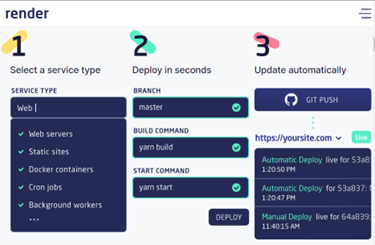
\includegraphics[scale=1.0]{slike/render.PNG} %veličina slike u odnosu na originalnu datoteku i pozicija slike
			\centering
			\caption{Render platfroma}
			\label{fig:render}
		\end{figure}
Prije prijave na „Render“ platformu i kreiranja poveznice prema našem repozitoriju, u korijenskoj mapi izvornog koda potrebno je kreirati "render.yaml" datoteku. Ta datoteka predstavlja „Blueprint spec“ - konfiguraciju potrebnu za izvođenje i puštanje aplikacije u pogon na „Render“ platformi.

Unutar datoteke potrebno je definirati tri servisa koji predstavljaju komponente aplikacije – „server“, „client“ i „db“.  Svaki servis, osim servisa vezanog u „PostrgeSQL“ bazu, mora sadržavati svojstva "type", "name" i "env". 

Servis vezan uz „PostrgeSQL“ bazu mora sadržavati samo svojstvo "name", a informacije za njegovo izvođenje dostupne su kroz već gotovi i dostupan servis „Render“ platforme. 
\begin{figure}[H]
			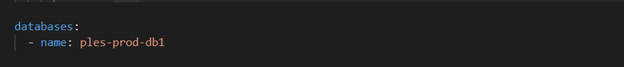
\includegraphics[scale=0.9]{slike/Slika2.PNG} %veličina slike u odnosu na originalnu datoteku i pozicija slike
			\centering
			\caption{Servis baze podataka}
			\label{fig:dbServis}
		\end{figure}

Kod preostalih dvaju servisa - jednog za "frontend", jednog za "backend" navedena svojstva postavljamo kako je prikazano na slikama \ref{fig:ServerServis} i \ref{fig:ClientServis}:

\begin{figure}[H]
			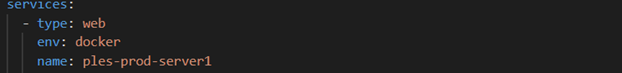
\includegraphics[scale=0.9]{slike/Slika3.PNG} %veličina slike u odnosu na originalnu datoteku i pozicija slike
			\centering
			\caption{Servis servera}
			\label{fig:ServerServis}
		\end{figure}

\begin{figure}[H]
			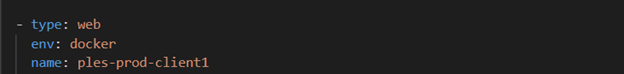
\includegraphics[scale=0.9]{slike/Slika4.PNG} %veličina slike u odnosu na originalnu datoteku i pozicija slike
			\centering
			\caption{Servis klijenta}
			\label{fig:ClientServis}
		\end{figure}

Svojstvo „env“, koje predstavlja okruženje izvođenja, potrebno je postaviti na „Docker“ čime definiramo izgradnju naše aplikacije kroz „Docker“ kontejnere.
Svaki definirani servis zapravo predstavlja informacije o „Docker image“ datotekama. Sadržaj tih datoteka uključuje kod komponenti, alate sustava, biblioteke i sve ostale postavke potrebne za izgradnju kontejnera potrebnih za izvođenje aplikacije.

Svaka „Docker image“ datoteka kreirana je koristeći skup naredbi definiran u datotekama naziva „Dockerfile" koje se nalaze u izvornom kodu aplikacije (jedna za „server“ - slika \ref{fig:ServerDoc}, jedna za „client“- slika \ref{fig:ClientDoc}). „Render“ iz tih datoteka dohvaća „startCommand“ svojstvo kojim se pokreće pojedini kontejner. 
\begin{figure}[H]
			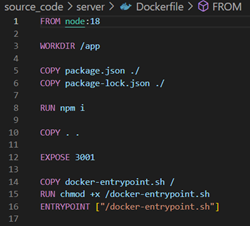
\includegraphics[scale=0.9]{slike/Slika5.PNG} %veličina slike u odnosu na originalnu datoteku i pozicija slike
			\centering
			\caption{Dockerfile server}
			\label{fig:ServerDoc}
			
		\end{figure}
\begin{figure}[H]
			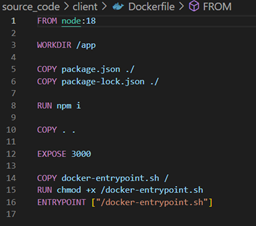
\includegraphics[scale=0.9]{slike/Slika6.PNG} %veličina slike u odnosu na originalnu datoteku i pozicija slike
			\centering
			\caption{Dockerfile klijent}
			\label{fig:ClientDoc}
		\end{figure}
Svojstvo „repo" kod oba servisa postavljamo na putanju na kojoj je dostupan repozitorij sa izvornim kodom aplikacije. Ovo svojstvo govori „Render“ platformi gdje se nalazi izvorni kod aplikacije koja će biti puštena u pogon.

Svojstvo „branch" postavljamo na „master" granu repozitorija definiranog pod "repo", dok svojstvom „rootDir" svakom servisu definiramo korijensku mapu unutar repozitorija gdje se nalazi sav kod potreban za izgradnju i izvođenje tog pojedinog servisa aplikacije. 

Svojstvo „buildFilter" potrebno je za svaki servis postaviti na uzorak putanje koji predstavlja lokacije datoteka unutar repozitorija čije bi izmjene na „master“ grani  trebale uzrokovati ponovnu izgradnju pojedinog servisa (redeployment).
\begin{figure}[H]
			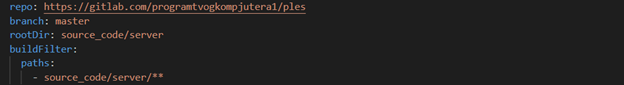
\includegraphics[scale=0.9]{slike/Slika7.PNG} %veličina slike u odnosu na originalnu datoteku i pozicija slike
			\centering
			\caption{Direkoriji servera}
			\label{fig:ServerRepo}
		\end{figure}
\begin{figure}[H]
			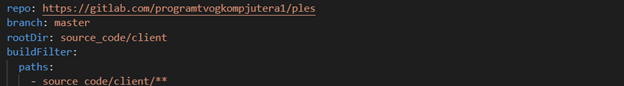
\includegraphics[scale=0.9]{slike/Slika8.PNG} %veličina slike u odnosu na originalnu datoteku i pozicija slike
			\centering
			\caption{Direktoriji klijenta}
			\label{fig:ClientRepo}
		\end{figure}

Ova svojstva zapravo omogućuju automatski redeployment samo onog dijela aplikacije kod kojeg su na „master“ grani uvedene nove promjene u odnosu na zadnji deploy.  

Uz dosad navedena svojstva, još je potrebno definirati varijable okruženja. 

„Render“ nudi mogućnost ovisnosti varijabli okruženja jednog servisa o svojstvima već gotovih „Render“ servisa. Varijable okruženja koje koristimo za spajanje „backend“ servisa na bazu podataka dohvaćamo preko definiranih svojstava „Render“ gotovog servisa za „PostgreSQL“ bazu podataka. Ostale varijable okruženja, koje ne bi smjele biti dostupne svima, stavljamo direktno na „Render“ platformu prije spremanja promjena.
\begin{figure}[H]
			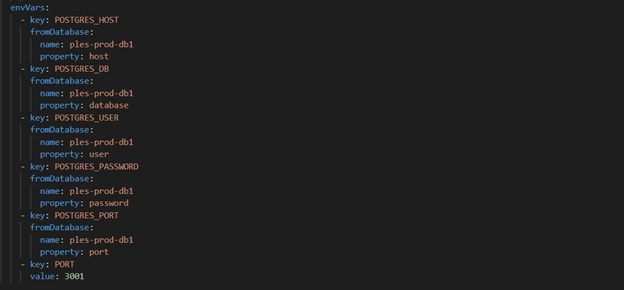
\includegraphics[scale=0.9]{slike/Slika9.PNG} %veličina slike u odnosu na originalnu datoteku i pozicija slike
			\centering
			\caption{Varijable okruženja za spajanje na bazu podataka}
			\label{fig:EnvDb}
		\end{figure}

Za korištenje već navedene platforme, prvo je potrebno napraviti račun te se prijaviti na adresi \url{https://dashboard.render.com/}. Nakon izrade računa u navigaciji „Render“ web aplikacije potrebno je odabrati „Blueprints" te "New Blueprint Instance" - u ovom koraku potrebno je izabrati repozitorij i granu na kojoj se nalazi naš izvorni kod aplikacije u čijem se korijenskom direktoriju nalazi gore opisana "render.yaml" datoteka. („Render“ platforma nudi unošenje podataka o vlastitom računu na „GitLab“ platformi i povezivanje s dostupnim repozitorijima). 

Nakon spremanja promjena, „Render“ web aplikacija povezana je s repozitorijem u kojem se nalazi izvorni kod aplikacije sa „render.yaml“ - slika \ref{fig:yaml} datotekom. „Render“ dohvaća i čita sadržaj te datoteke te na temelju definirane konfiguracije pušta aplikaciju u pogon.
\begin{figure}[H]
			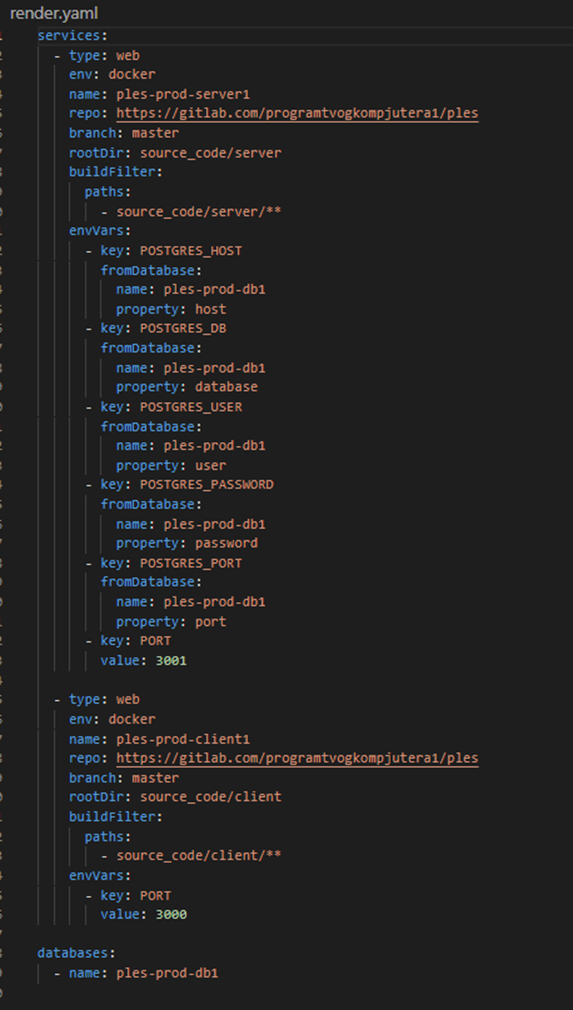
\includegraphics[scale=0.7]{slike/Slika10.PNG} %veličina slike u odnosu na originalnu datoteku i pozicija slike
			\centering
			\caption{Prikaz cijele "render.yaml" datoteke}
			\label{fig:yaml}
		\end{figure}

Aplikacija puštena u pogon se može pokrenuti na adresi \url{https://ples-prod-client1-goj4.onrender.com/}.

			\eject 
			
			
			\eject 
